\section{Opgaver fra kapitel 0}


\subsection{Opgave 1}
Bestem den lineære sammenhæng $y = ax + b$, når vi kender to punkter A(1,3) og B(2,4) på den rette linje.

For at bestemme den lineære sammenhæng når vi kendet 2 punkter på den rette linje skal vi altså bestemme forskriften for den linje som går igennem disse punkter. Når vi bestemmet forskriften af en ret linje der går igennem 2 punkter bestemmer vi først hældningen ud fra Theorem \ref{a}. Vi vælger punktet A(1,3) som vores $(x_1,y_1)$ og B(2,4) som vores $(x_2,y_2)$ og får hældningen

\begin{align*}
a = \frac{y_2-y_1}{x_2-x_1} = \frac{4-3}{2-1} = \frac{1}{1} = 1
\end{align*}

Hældningen af den rette linje der går gennem punkterne A og B er dermed $a = 1$.

Det sidste man skal bruge for at bestemme forskriften af en ret linje der går gennem 2 punkter er at beregne linjens skæring med y aksen, b. Vi bestemmer skæringen med y-aksen ved brug at Theorem \ref{b}. Vi vælger punktet A(1,3) som vores $(x,y)$ og får

\begin{align*}
b = y-ax = 3-1\cdot 1= 2 
\end{align*}

Den rette linje der går gennem punkterne A og B skærer dermed y-aksen ved 2.

Forskriften for den rette linje som går igennem punterne A og B er dermed

\begin{align*}
y = 1x + 2 = x + 2
\end{align*}

Vi kan eftertjekke ved at indtegne den rette linje med forskriften $y = x+2$ i geogebra samt punkterne A(1,3) og B(2,4) og se om punkterne ligger på den rette linje. Som vi kan se på billedet nedenfor ligger punkterne A(1,3) og B(2,4) på den rette linje med forskriften $y = x+2$ så vi ved at vi har bestemt forskriften korrekt.

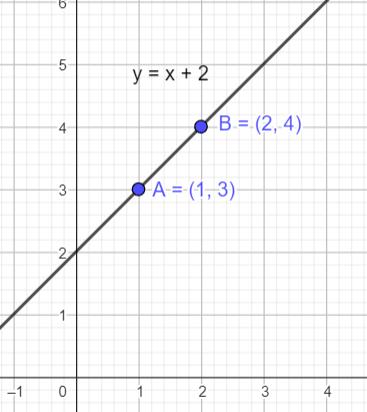
\includegraphics[scale=0.7]{img_13}

\subsection{Opgave 2}
Bestem den lineære sammenhæng $y=ax+ b$, når vi kender to punkter A(1,-3) og B(2,4) på den rette linje.

Vi gør præcis som i opgave 1 hvor vi først bestemmer hældningen af den rette linje som går igennem punkterne A(1,-3) og B(2,4) og derefter bestemmer den rette linjes skæring med y-aksen.

Vi vælger A(1,-3) til $(x_1,y_1)$ og B(2,4) til $(x_2,y_2)$ og bruger formlen i Theorem \ref{a} til at beregne hældningen

\begin{align*}
a = \frac{y_2-y_1}{x_2-x_1} = \frac{4-(-3)}{2-1} = \frac{4+3}{1} = \frac{7}{1} = 7
\end{align*}

Hældningen af den rette linje som går gennem punkterne A og B er dermed $a = 7$.

Vi vælger punktet A(1,-3) som $(x,y)$ og bruger formlen fra Theorem \ref{b} til at beregne den rette linjes skæring med y-aksen.

\begin{align*}
b = y-ax = -3 - 7\cdot 1 = -3-7 = -10
\end{align*}

Den rette linje som går igennem punkterne A og B skærer altså y-aksen i -10.

Forskriften for den rette linje bliver dermed 
\begin{align*}
y = 7x-10
\end{align*}

Vi kan eftertjekke ved at indtegne den rette linje med forskriften $y = 7x-10$ i geogebra samt punkterne A(1,-3) og B(2,4) og se om punkterne ligger på den rette linje. Som vi kan se på billedet nedenfor ligger punkterne A(1,-3) og B(2,4) på den rette linje med forskriften $y = 7x-10$ så vi ved at vi har bestemt forskriften korrekt.

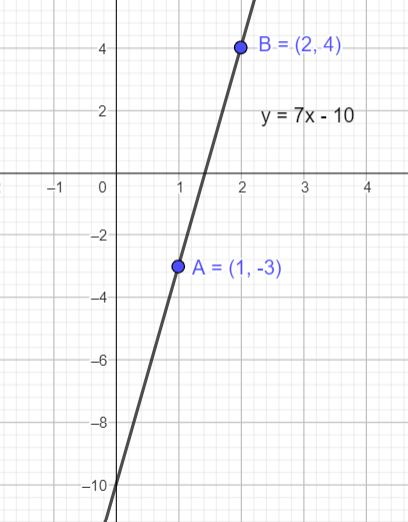
\includegraphics[scale=0.6]{img_14}



\subsection{Opgave 5}
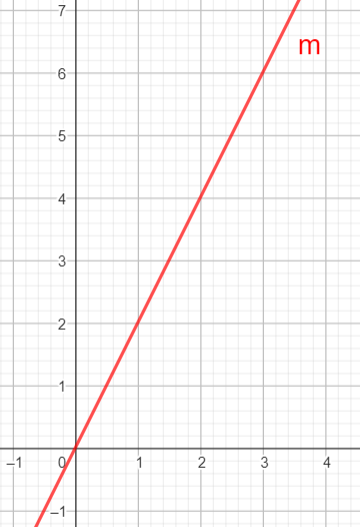
\includegraphics[scale=0.6]{img_15}

Bestem ved aflæsning af grafen a og b for den rette linje m.

Vi bestemmer hældningen a ved at gå 1 ud ad x-aksen og derefter gå op eller ned til vi støder på den rette linje m. Det stykke vi har bevæget os op eller ned indtil vi støder på linjen er hældningen a. Vi aflæser hældningen til $a = 2$.

For at bestemme b så aflæser vi y-værdien der hvor den rette linje skærer y-aksen. I dette tilfælde aflæser vi $b=0$.

Svarene er illustreret på nedenstående billede.

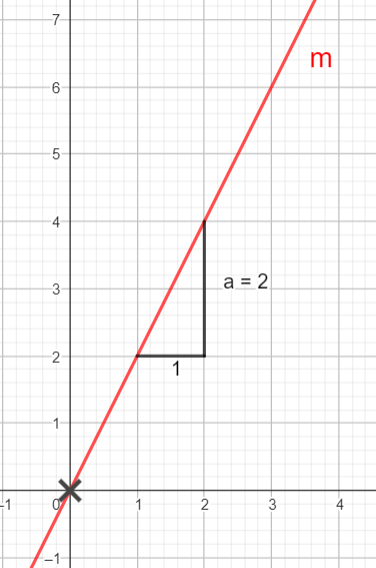
\includegraphics[scale=0.6]{img_16}



\subsection{Opgave 8}

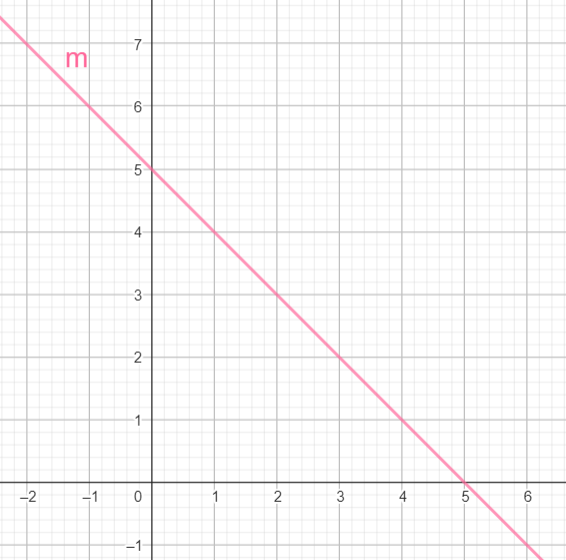
\includegraphics[scale=0.6]{img_17}

Bestem ved aflæsning af grafen a og b for den rette linje m.

Vi bestemmer hældningen a ved at gå 1 ud ad x-aksen og derefter gå op eller ned til vi støder på den rette linje m. Det stykke vi har bevæget os op eller ned indtil vi støder på linjen er hældningen a. Vi aflæser hældningen til $a = -1$.

For at bestemme b så aflæser vi y-værdien der hvor den rette linje skærer y-aksen. I dette tilfælde aflæser vi $b=5$.

Svarene er illustreret på nedenstående billede.

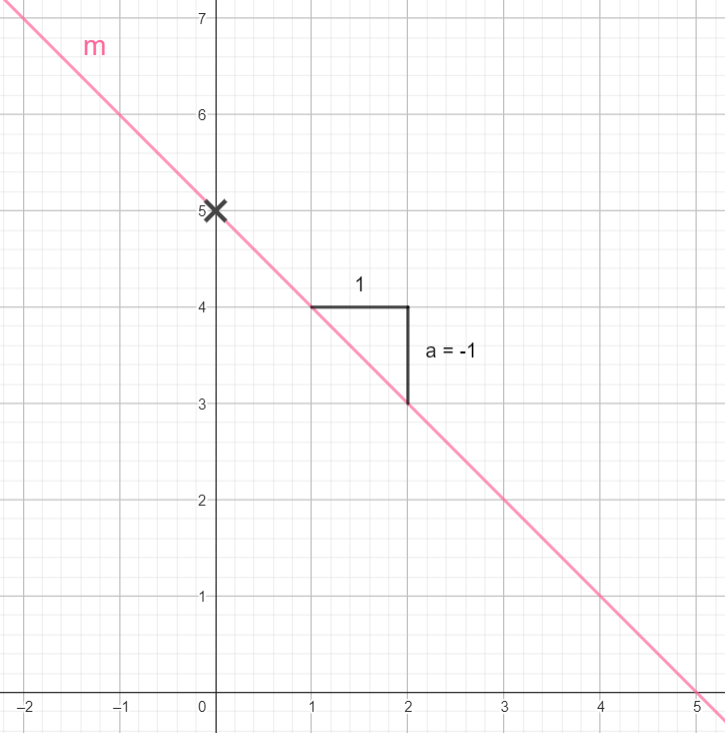
\includegraphics[scale=0.6]{img_18}

